% !TEX root = main.tex
\chapter{Introduzione}
Nel progetto sono stati affrontati alcuni dei vari problemi che riguardano l'intelligenza artificiale. In questa relazione spiegheremo quali soluzioni sono state adottate, i vantaggi e gli svantaggi e alcuni miglioramenti che possono esser fatti al nostro progetto

\section{Strategie}
Per svolgere il progetto di IA-LAB sono state implementate 4 strategie in maniera incrementale:
\begin{itemize}
  \item FIFO WAIT: la strategia usa la politica fifo come politica di scelta degli ordini. 
  \item FIFO PRO: Simile alla precendente, ma in caso di ostacolo che non permette di servire un ordine, l'ordine viene messo al fondo.
  \item LOW PENALITY: strategia che si basa sulla penalità per effettuare la scelta dell'ordine.
  \item HARD: a differenza delle altre 3 strategia, questa permette di gestire più ordini in contemporanea. Come la precedente si basa sulle penalità.
\end{itemize}

Ogni strategia è stata suddivisa in fasi dove ogni fase si occupa di uno specifico sotto-problema. Questa suddivisione ci ha permesso sia uno sviluppo incrementale all'interno della stessa strategia, sia tra strategie diverse, dove è bastato andare a sviluppare in modo più articolato una fase oppure nell'inserire nuove fasi.
Nelle prime due strategia come astrazione utilizzeremo il concetto di coda. Gli ordini verranno inseriti in coda e prelevati dalla testa, quindi prelevati in ordine crescente di step.

\subsection{Astar}
Tutte le strategia utilizzano il modulo Astar per pianificare dei piani che permettano al nostro robot di spostarsi da un punto A a un punto B. Il punto A è la posizione del robot al momento della pianificazione mentre il goal (il punto B) è dato dalla cella destinazione. La cella destinazione può essere un dispenser, un cestino o un tavolo. Il modulo astar calcolerà quali sono i 4 punti di accesso alla nostra destinazione e si fermerà non appena arriverà a uno di esso.

Il modulo A* può terminare fornendo un piano, oppure può fallire. Per memorizzare il piano creato vengono usate due strutture:

\begin{lstlisting}
(deftemplate plane 
	(slot plane-id) 
	(multislot pos-start) 
	(multislot pos-end) 
	(slot direction) 
	(slot cost) 
	(slot status (allowed-values ok failure))
)
\end{lstlisting}
\begin{lstlisting}
(deftemplate step-plane 
	(slot plane-id)
	(slot action)
	(slot direction)
	(multislot pos-start)
	(slot father)
	(slot child)
)
\end{lstlisting}

La struttura step-plane indica i vari passi per eseguire il piano plane. I piani vengono memorizzati in modo tale che il robot non debba ripianificare più volte uno stesso percorso. Vengono memorizzati solo i piani principali; nel caso in cui un piano fallisca il piano "riparatore" non viene memorizzato.

\chapter{Strategie}
\section{Strategia FIFO WAIT}
La prima strategia che illuestreremo è la FIFO WAIT. \'E una strategia molto semplice, dove il primo ordine che arriva è l'ordine che viene servito. Vi sono vari casi per completare un ordine:\begin{itemize}
  \item Ordine Accepted: un ordine di questo tipo verrà completato solo quando verranno consegnate al tavolo tutte le consumazioni richieste.
  \item Ordine Delayed: un ordine di questo tipo verrà completato solo quando verranno consegnate al tavolo tutte le consumazioni richieste. Rispetto al caso precedente le consumazioni non potranno esser consengate fin quando il tavolo non verrà pulito e le consumazioni buttate nel cestino.
  \item Ordine Finish: un ordine di questo tipo verrà completato solo quanto verrà pulito il tavolo e il robot butterà lo sporco nei vari cestini.
\end{itemize}
\newpage

\begin{figure}[htp]
  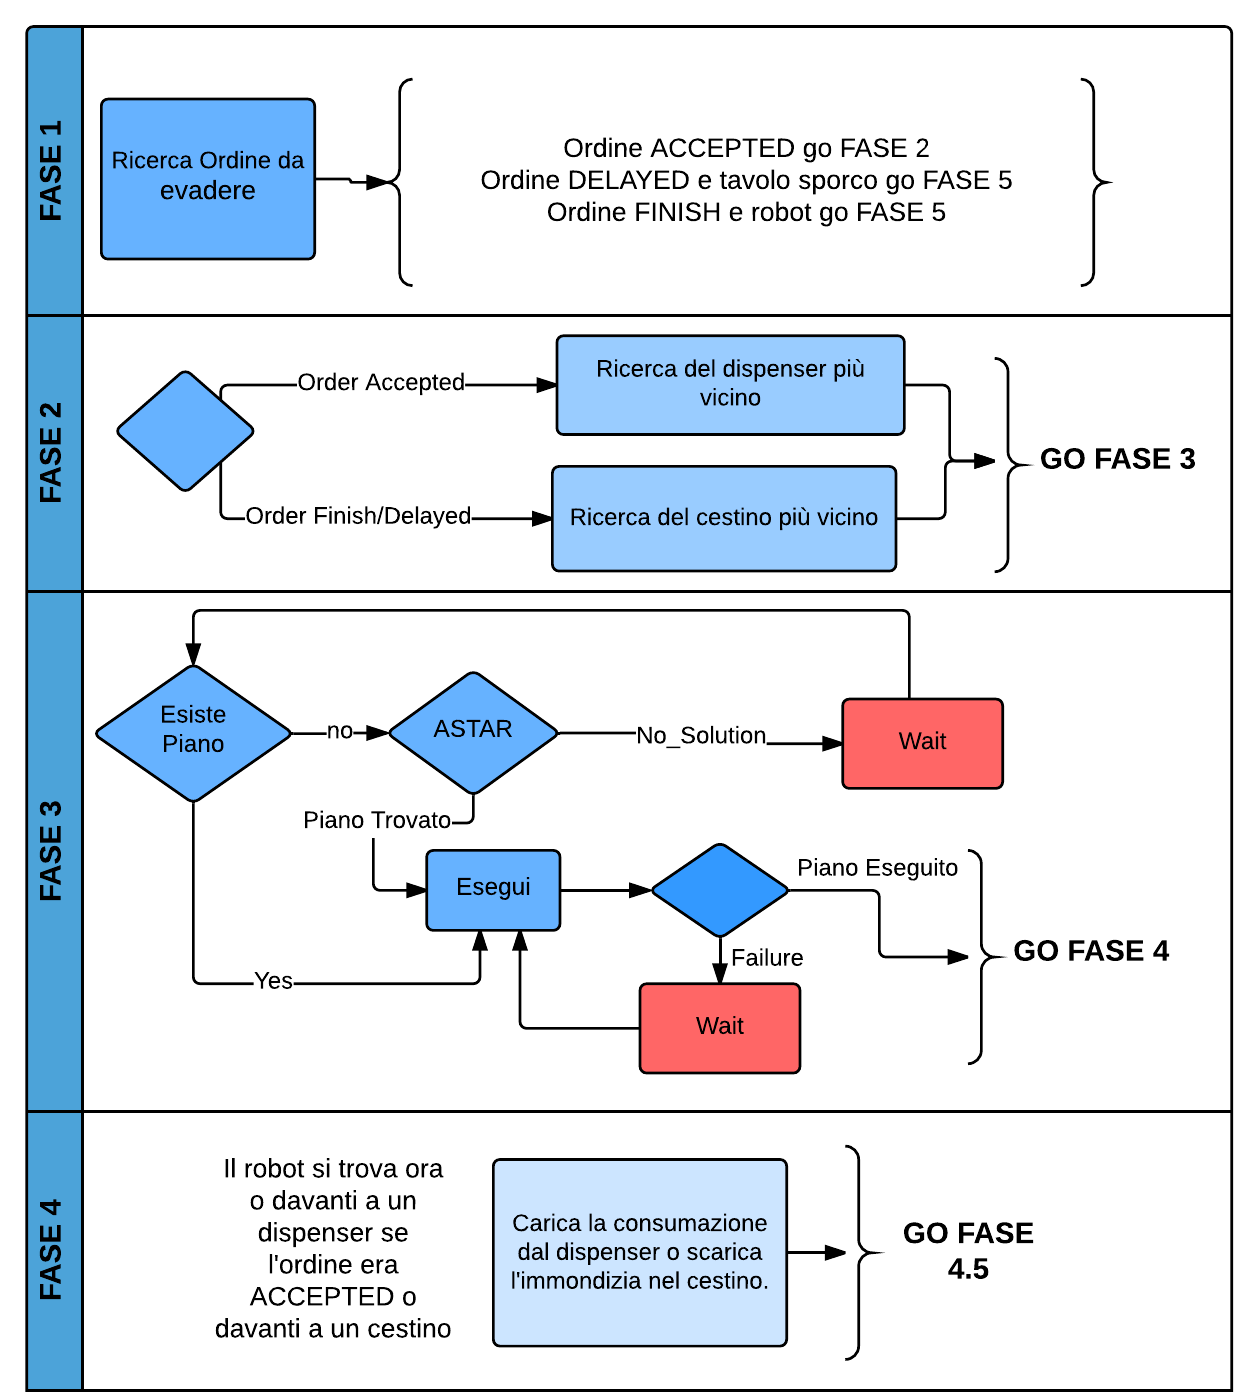
\includegraphics[width=\textwidth]{schema-fifo-wait1.png}
  \caption{Schema Fifo Wait}
  \label{fig:figure1}
\end{figure}

\begin{figure}[htp]
  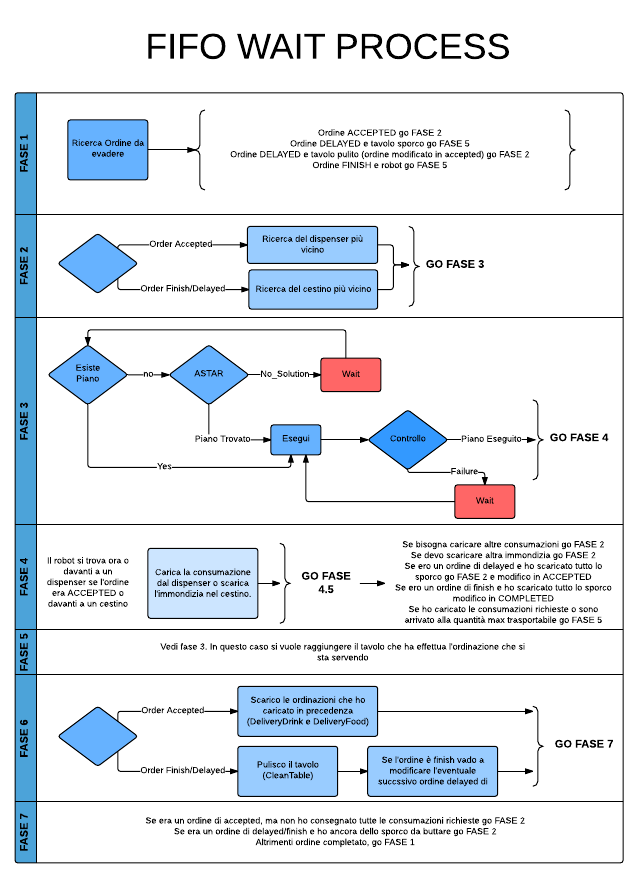
\includegraphics[width=\textwidth]{schema-fifo-wait2.png}
  \caption{Schema Fifo Wait}
  \label{fig:figure2}
\end{figure}

Come possiamo vedere dallo schema abbiamo suddiviso la nostre strategia in 7 fasi:
\begin{itemize}
  \item Fase 1: Nella prima fase viene individuato quale sarà l'ordine da servire. Ipotizzando di avere una coda in cui gli inserimenti vanno in coda e i prelievi dalla testa, l'ordine da evadere sarà l'ordine arrivato da più tempo cioè quello che ha un valore di step più basso.
  \item Fase 2: In questa fase si andrà ad individuare quale sarà il cestino o il dispenser presso il quale il nostro robot dovrà recarsi. La ricerca del cestino o del dispenser dipene dal tipo di ordine.
  \item Fase 3: In questa fase il robot arriverà alla destinazione prefissata. Per far ciò deve prima calcolare un piano con A* e poi eseguirlo. Il piano viene calcolato solo se non ne esiste già uno. In caso A* non trovi soluzione il robot esegue una wait e prova a ricalcolare A* fin quando non trova una soluzione.
  Quando il robot ha un piano per raggiungere la sua destinazione lo esegue. Nel caso in cui il piano fallisca il robot esegue una wait e prova a rieseguirlo.
  \item Fase 4: Il robot a seconda dell'ordine che sta servendo si troverà davanti un dispenser per caricare delle consumazioni (ordine accepted) oppure davanti a un cestino per buttare lo sporco (ordine delayed o finish).
  \item Fase 4.5: Questa è fase di controllo in cui il robot decide a seconda dell'ordine cosa deve fare. Per esempio se era un ordine accepted e ha caricato solo i 'food' e gli mancano i 'drink' dovrà ritornare alla fase 2; analogamente se era un ordine di finish o delayed e deve ancora buttare dello sporco.
  \item Fase 5: Identica alla fase 3 tranne per il fatto che la destinazione sarà un tavolo.
  \item Fase 6: Il robot in questa fase si trova in una posizione in cui può operare sul tavolo. Nel caso di ordine accepted rilascio tuttle le consumazioni caricate; in caso di ordine finish o delayed pulisco il tavolo.
  \item Fase 7: In questa fase controllo se l'ordine può essere considerato completato.
\end{itemize}

\subsection{Vantaggi e Svantaggi}
Vantaggio di questa strategia è sicuramente la semplicità e l'intuibilità con la quale il sistema funziona. L'idea di questa strategia, oltra alla politica di evasione degli ordini che può essere cambiata in qualsiasi momento andando solo a modificare la fase 1, è quella che il mondo è dinamico e lo è con una certa frequenza. 

\begin{wrapfigure}{r}{0.33\textwidth} 
    \centering
    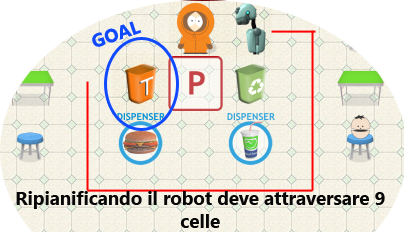
\includegraphics[width=0.33\textwidth]{Problema1_fifo_wait}
\end{wrapfigure}

L'assunzione dalla quale siamo partiti è che le persone si spostano e si spostano molto frequentemente. Da questo risulta evidente che se per arrivare in una determinata posizione incontro un ostacolo (una persona) la mossa più conveniente è quella di aspettare.
Se prendiamo in considerazione le teorie di Rodney Brooks in cui afferma che un comportamento intelligente è attribuibile da un osservatore esterno che vede l'agente interagire con l'ambiente, allora in alcune circostanze il nostro agente potrebbe non dimostrare tale comportamento intelligente. Se una persona rimane, anche se per pochi step in una posizione lungo il percorso dell'agente, il nostro agente invece di aggirarla e dimostrare un comportamento intelligente continuerà a provare a muoversi lungo la sua direzione fin quando la persona non si sarà spostata. 

\begin{wrapfigure}{l}{0.25\textwidth} 
    \centering
    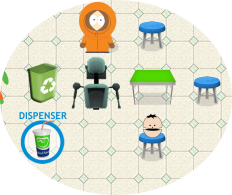
\includegraphics[width=0.25\textwidth]{Problema2_fifo_wait}
\end{wrapfigure}

Questo comportamento porta anche a situazioni di deadlock. Essendo in un ambiente simulato anche le persone non hanno un comportamento intelligente, supponendo che una persona si vuole spostare in direzione sud e il robot in direzione nord si arriva in una situazione di stallo. Per ovviare a questa problematica abbiamo implementato la strategia FIFO PRO.

\section{Strategia FIFO PRO}
La strategia FIFO PRO è un estensione della strategia FIFO WAIT per risolvere il "problema" riscontrato precedentemente. I concetti chiave che differenziano questa strategia dalla precendente sono 2:
\begin{itemize}
  \item ripianificazione nel caso un piano fallisca
  \item possibilità di cambiare l'ordine da servire se ci accorgiamo che non è possibile completarlo.
\end{itemize}

Il primo punto comporta delle modifiche nello schema visto in precedenza nella fase 3 e nella fase 5, ovvero nelle fasi delle ricerca ed esecuzione del piano. La figura \ref{fig:figure3} ci mostra le modifiche.

\begin{figure}[htp]
  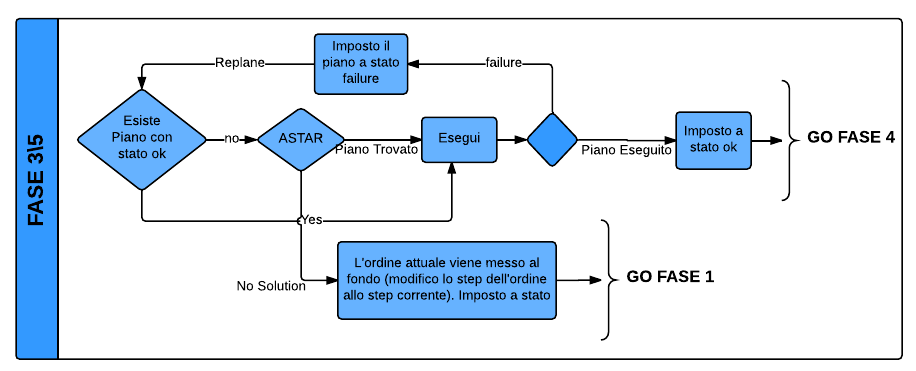
\includegraphics[width=\textwidth]{Fase3-FIFO-PRO}
  \caption{Fase 3 e 5 della strategia FIFO PRO}
  \label{fig:figure3}
\end{figure}

\newpage
\begin{wrapfigure}{r}{0.25\textwidth} 
    \centering
    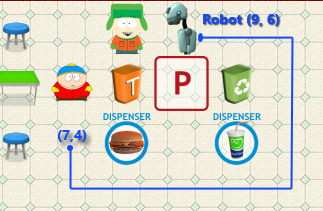
\includegraphics[width=0.25\textwidth]{Problema1_fifo_pro}
\end{wrapfigure}

Più complicate le conseguenze del secondo punto, che sono strettamente legate alla pianificazione. La pianificazione non trova sempre una soluzione. Nel caso in cui astar non riesca a trovare un percorso per raggiungere la nostra destinazione cambiamo l'ordine da servire. Questo comporta che l'ordine corrente verrà messo al fondo della nostra coda ordini e sarà servito successivamente. Questo commporta alcuni problemi che hanno complicato la stratgia FIFO PRO rispetto la precedente, e che saranno comuni anche alle successive strategie. 

La strategia FIFO WAIT aveva un grosso vantaggio: ogni volta che si serve un nuovo ordine sicuramente l'agente si trova nello stato adatto per iniziare a servirlo. 
Questo significa che l'agente non ha nè sporco nè consumazioni a bordo. Questa sicurezza non si ha nella strategia FIFO PRO. Supponiamo che un agente stia servendo un ordine finish e debba andare al cestino per liberarsi dallo sporco ma sfortunatamente il cestino non ha punti d'ingresso perchè occupati da persone, questo ordine verrà abbandonato e inserito al fondo e verrà recuperato il successivo ordine. Se il successivo ordine è un accepted non potrò subito avviare le operazioni per servirlo, ma dovrò sempre liberarmi dello sporco.

Nella fase 1 si ha un dispatcher che indica, a seconda dello stato dell'agente e dell'ordine, l'azione da compiere. La figura \ref{fig:figure4} mostra la fase 1 della strategia FIFO PRO.

\begin{figure}[htp]
  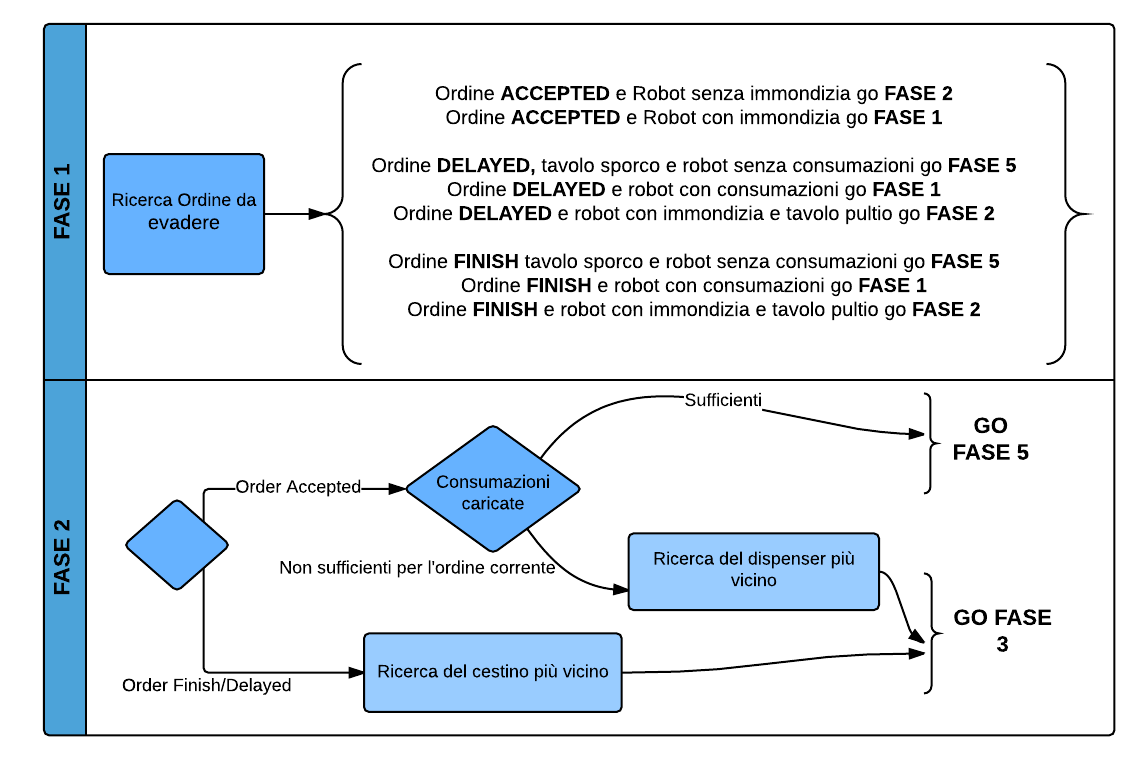
\includegraphics[width=\textwidth]{FIFO_PRO_fase1-2}
  \caption{Fase 1 e 2 della strategia FIFO PRO}
  \label{fig:figure4}
\end{figure}

Rimescolando gli ordini può succedere che ordini accepted vengano completati in ordine diverso dal quale siano arrivati. Nella stategia FIFO WAIT si era sicuri che una volta caricate le consumazioni dai dispenser, quelle consumazioni sarebbero state consegnata al tavolo che le aveva richieste. Nella strategia FIFO PRO questo non avviene. Supponendo di aver caricato dai dispenser un tot di consumazioni e che il robot non riesca ad arrivare al tavolo, il successivo ordine di accepted che verrà prelevato dalla coda potrebbe non aver bisogno di tornare ai dispenser (o di tornarci parzialmente), in quanto il robot ha già a bordo le consumazioni dell'ordine precedente. Si è dovuto implementare un meccanismo che permetta di capire al robot se e quanto deve caricare dai dispenser.

Altra piccola modifica avviene nella fase 6. Nella strategia FIFO WAIT gli ordini di tipo finish erano sicuramente eseguiti prima degli ordini di tipo delayed (questo comportava di andare a modificare l'ordine delayed in accepted una volta pulito il tavolo). Nella strategia FIFO PRO questo non è sempre vero, è possibile che un ordine finish venga rimesso al fondo della nostra coda e verrà eseguito un ordine di delayed (ovviamente ci riferiamo a ordini sullo stesso tavolo). In questo caso se l'ordine delayed riesce con successo a pulire il tavolo, il sistema dovrà settare come completata anche l'ordine finish.

Nella fase 7 inoltre quando il robot svuota l'immondizia bisogna andare a settare a completato tutti gli ordini finish che sono stati rimessi in coda perchè il dispenser era occupato.

\begin{figure}[htp]
  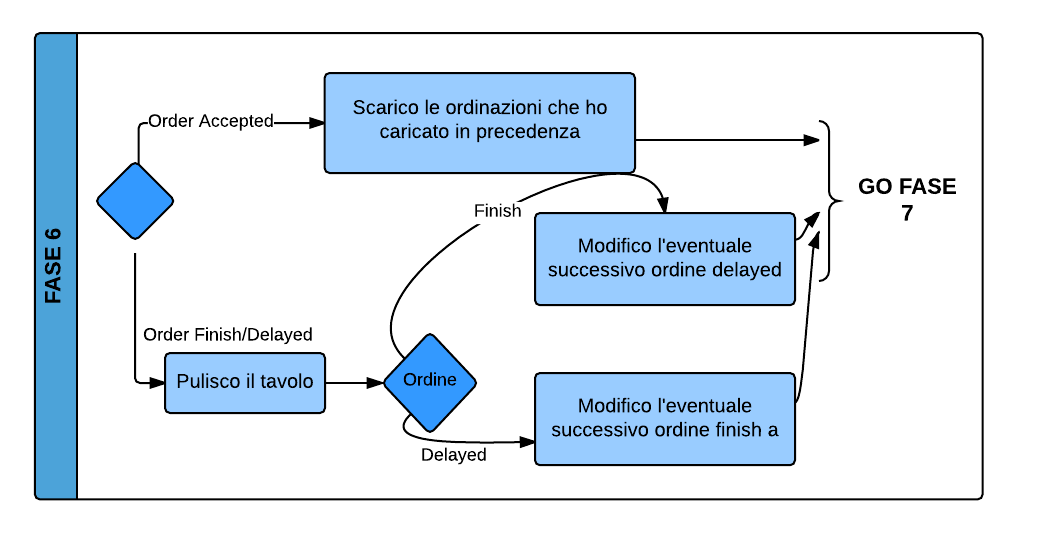
\includegraphics[width=\textwidth]{FIFO_PRO_fase6}
  \caption{Fase 6 della strategia FIFO PRO}
  \label{fig:figure5}
\end{figure}

\subsection{Vantaggi e Svantaggi}
Il sistema riesce dinamicamente a servire i vari ordini ripianificando i percorsi o cambiando gli ordini da servire. Obiettivo di questa strategia è rendere il sistema più robusto e flessibile. Utilizzando questa strategia rispetto alla precedente non è detto che si migliori l'efficienza del sistema.
Anche utilizzando questa strategia il sistema potrebbe rimanere bloccato, si veda la figura \ref{fig:figure6}. Si potrebbe ulteriormente ottimizzarla andando a imporre un numero di fallimenti massimo per arrivare a una specifica posizione; arrivati a tale limite l'ordine viene rimpiazzato dal successivo.

\begin{SCfigure}[]
\centering
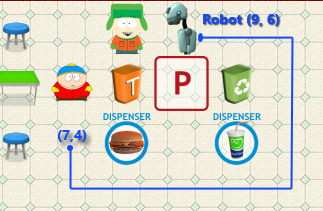
\includegraphics[width=0.40\textwidth]{Problema1_fifo_pro}
\caption{In questo esempio il robot vuole arrivare al TD e continuerà a spostarsi dalla cella (9,6) alla (7,4) e viceversa. Ricordiamo che il robot del mondo conosce solo lo stato delle 9 celle adiacenti a lui e le posizioni dei dispenser e dei tavoli. Quando si trova nella cella (7,4) non sa che nella (9,5) c'è una persona e quindi astar pianifica verso quella destinazione.}
\label{fig:figure6}
\end{SCfigure}

\section{Strategia LOW PENALITY}
La strategia LOW PENALITY si differenzia dalla precedente soprattutto per la Fase 1, ovvero per la ricerca dell'ordine da evadere. Si abbandona la politica FIFO per individuare e servire l'ordine che a ogni step porterebbe una penalità maggiore. Ogni qual volta arriva un ordine, viene calcolata la relativa penalità. Quando bisogna scegliere un ordine si sceglie quello con penalità maggiore. L' obiettivo è quello di minimizzare la penalità.
Altra differenza con le precedenti strategia sta nella gestione dell'ordine accepted. Nelle precedenti strategie l'ordine viene evaso completamente. In questa strategia si vuole minimizzare le penalità, quindi se un ordine ha richiesto 3 food e 3 drink, l'agente consegnerà le consumazioni secondo la sua massima capienza. Consegnate le consumazioni l'ordine o è stato completato o viene rimesso negli ordini da evadere aggiornando le consumazioni (e le penalità) in base a quelle già consegnate.

\subsection{Vantaggi e Svantaggi}
Obiettivo di questa strategia è quella di minimizzare le penalità rispetto alle strategia precedenti. Vedremo nella sezione Analisi Strategia se i risultati sono stati raggiunti. Gli svantaggi sono i medesimi della strategia FIFO PRO.

\section{Strategia HARD}
La strategia HARD è la più complessa e permette di servire più tavoli in contemporanea. In comune con la strategia precedente ha la ripianificazione nel caso il piano calcolato fallisca, e il cambio dell'ordine corrente per un altro nel caso non si riesca a trovare un piano per arrivare a destinazione.
Iniziamo a vedere il meccanismo con il quale viene scelto l'ordine da evadere (FASE 1).

\begin{figure}[htp]
  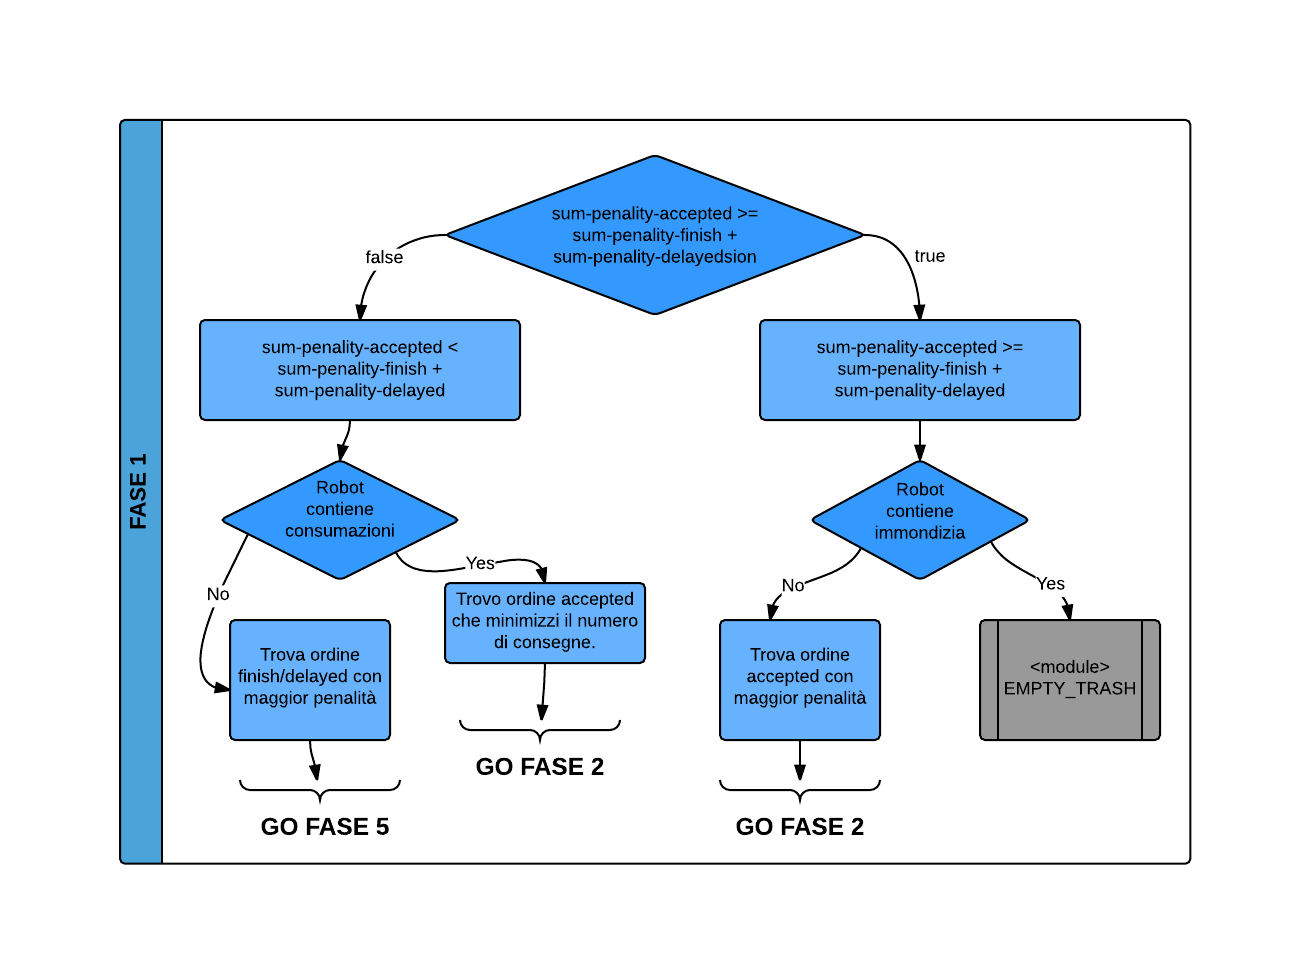
\includegraphics[width=\textwidth]{HARD_fase1}
  \caption{Fase 1 della strategia HARD}
  \label{fig:figure7}
\end{figure}

\begin{equation}
\label{eqn:ordine}
Ordine=\max(x1,x2+x3).
\end{equation}
\[
x1=\sum_{k=1}^n Ordine_\textup{accepted,k}(pen).
\]\[
x2=\sum_{k=1}^n Ordine_\textup{delayed,k}(pen).
\]\[
x3=\sum_{k=1}^n Ordine_\textup{finish,k}(pen).
\]

Dalla formula \eqref{eqn:ordine} si deduce qual'è l'insieme di ordini che a ogni istante di tempo introducono più penalità nel sistema. Una volta individuato questo insieme si cerca al suo interno l'ordine con penalità maggiore. Tale ordine verrà servito.
In alcuni casi il robot prima di servire tale ordine deve compiere delle altre operazion:  
\begin{itemize}
  \item l'ordine da evadere è una finish o delayed ma ho delle consumazioni a bordo, il robot deve consegnare le consumazioni che ha prima di servire l'ordine finish o delayed. Di conseguenza bisogna cercare uno o più ordini accepted. L'idea che sta alla base della ricerca in questo caso è quella di trovare l' ordine o gli ordini che minimizzino il numero di consegne. Se il robot si trova in una situazione di 1drink e 1food preferirà consegnare le consumazioni a un singolo tavolo invece che a due diversi.
  \item l'ordine da evadere è un accepted ma il robot ha sporco a bordo, il sistema forza il robot a recarsi ai cestini.
\end{itemize}

La fase 2 e 3 sono quasi identiche alle precedenti. La fase 2 viene esegita solo nel caso di ordini accepted, quindi si ricercherà solo il dispenser più vicino al robot. 

\begin{figure}[htp]
  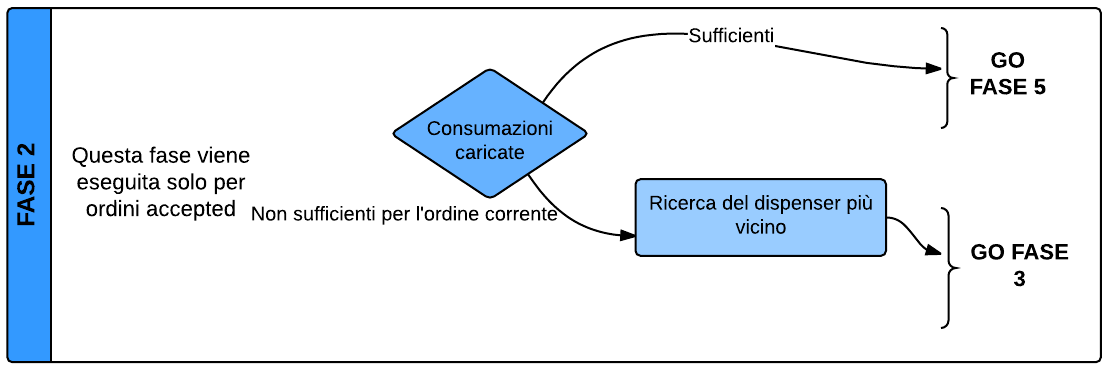
\includegraphics[width=\textwidth]{HARD_fase2}
  \caption{Fase 2 della strategia HARD}
  \label{fig:figure8}
\end{figure}

Nella fase 4, ovvero il caricamento dai dispenser delle consumazioni, abbiamo introdotto la possibilità di caricare le consumazioni per più ordini. Quando il robot arriva a un dispenser carica le consumazioni per l'ordine corrente. Se ha ancora spazio a disposizione e vi sono conumazioni di altri ordini da poter caricare vengono caricate fino al raggiungimento della capacità massima. 
La fase 4.5 è molto più semplice delle precedenti. Il fatto di trattare e gestire la pulizia dei tavoli nel modulo EMPTY TRASH ha reso meno complicate alcune fasi.

\begin{figure}[htp]
  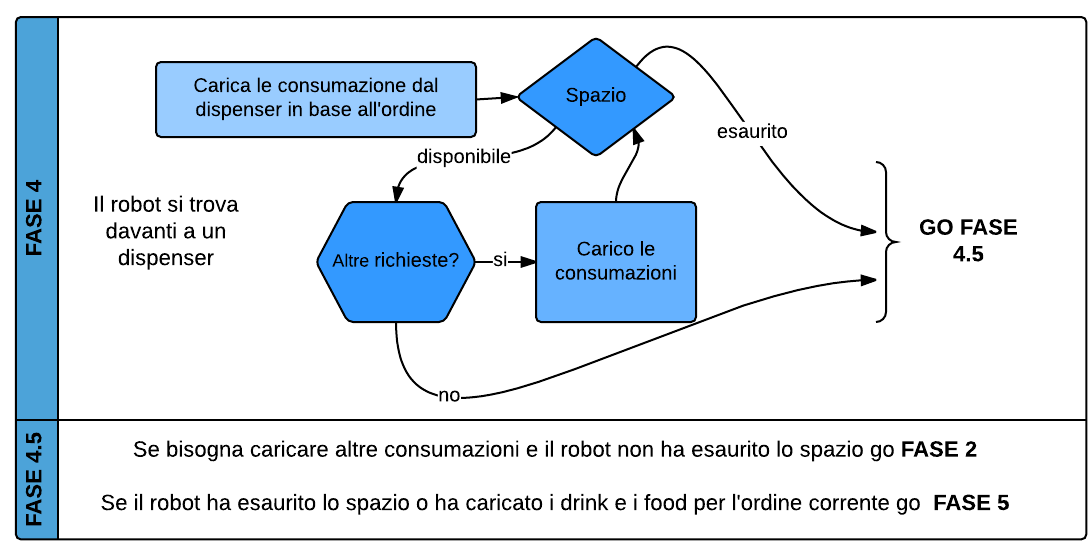
\includegraphics[width=\textwidth]{HARD_fase4_45}
  \caption{Fase 4 e 4.5 della strategia HARD}
  \label{fig:figure9}
\end{figure}

La fase 5 ovvero la ricerca e l'esecuzione del piano per arrivare al tavolo rimane immutata, e non la descriviamo nuovamente.


Nella fase 6 si consegnano le consumazioni al tavolo se era un ordine di accepted o si pulisce il tavolo se era un ordine di finish o delayed. 
Nel primo caso potrebbe capitare che l'ordine non risulti completamente evaso, e come nella strategia LOW PENALITY, quest'ordine torna nella lista di ordini da evadere aggiornando le consumazioni da portare in base a quelle già consegnate.
Nel caso sia un ordine di finish oltre a pulire il tavolo l'ordine viene impostato come completato, cosa che non accadeva nelle altre strategie.
Nel caso sia un ordine di delayed l'ordine viene impostato ad accepted e torna nella lista di ordini da evadere. In entrambi i casi il robot ha dello sporco a bordo, ma sarà la fase 1 della strategia che indicherà al robot di andare ai cestini.

\begin{figure}[htp]
  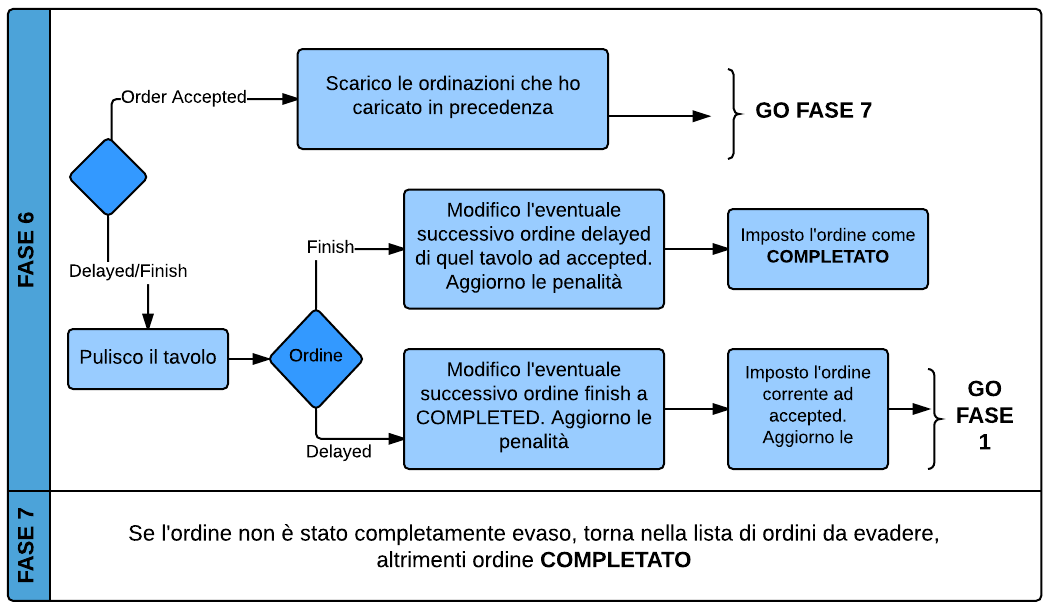
\includegraphics[width=\textwidth]{HARD_fase6-7}
  \caption{Fase 6 e 7 della strategia HARD}
  \label{fig:figure10}
\end{figure}

\subsection{Modulo EMPTY TRASH}
Questo modulo si occupa di liberare dallo sporco il robot. A differenza delle altre strategia, che ogni volta che si puliva un tavolo si cercava anche di liberarsi dello sporco, in questa la pulizia avviene soltanto in un caso (vedi \ref{fig:figure7}):
\begin{itemize}
\item l'ordine da evadere è un accepted ma il robot ha sporco a bordo, il sistema forza il robot a recarsi ai cestini.
\end{itemize}

\subsection{Checkfinish}